\documentclass[smaller,pdf,svgnames]{beamer}

\usepackage{color}
\usepackage{dsfont}
\usepackage{multimedia}

\useinnertheme{circles}
\newenvironment{proenv}{\only{\setbeamercolor{local structure}{fg=green}}}{}
\newenvironment{conenv}{\only{\setbeamercolor{local structure}{fg=red}}}{}

\usepackage{subfigure}

\title {A Genetic algorithm overview}
\author[Thomas Badie \and Victor Lenoir \and Pierre Parutto]{Thomas Badie\\Victor Lenoir\\Pierre Parutto}
\institute{}

\usetheme{Warsaw}

\usecolortheme[rgb={.25,.57,.29}]{structure}
\usepackage{algorithm}

\usepackage{algorithmicx}
\usepackage[noend]{algpseudocode}
%\setbeamercolor*{palette primary}{use=structure,fg=white,bg=mypurple}
\newcommand*\Let[2]{\State #1 $\gets$ #2}
\algrenewcommand\alglinenumber[1]{
    {\sf\footnotesize\addfontfeatures{Colour=888888,Numbers=Monospaced}#1}}
\algrenewcommand\algorithmicrequire{\textbf{Precondition:}}
\algrenewcommand\algorithmicensure{\textbf{Postcondition:}}



%% To get the page numbering clean.
\defbeamertemplate*{footline}{shadow theme}
{%
  \leavevmode%
  \hbox{\begin{beamercolorbox}[wd=.5\paperwidth,ht=2.5ex,dp=1.125ex,leftskip=.3cm plus1fil,rightskip=.3cm]{author in head/foot}%
    \usebeamerfont{author in head/foot}\insertframenumber\,/\,\inserttotalframenumber\hfill\insertshortauthor
  \end{beamercolorbox}%
  \begin{beamercolorbox}[wd=.5\paperwidth,ht=2.5ex,dp=1.125ex,leftskip=.3cm,rightskip=.3cm plus1fil]{title in head/foot}%
    \usebeamerfont{title in head/foot}\insertshorttitle%
  \end{beamercolorbox}}%
  \vskip0pt%
}

% To do not have the summary on each slide.
\setbeamertemplate{headline}{}

\begin{document}

\begin{frame}
  \maketitle
\end{frame}

\begin{frame}{Table of contents}
  \tableofcontents
\end{frame}

\section{A general overview}

\begin{frame}
  \frametitle{Summary}
  \tableofcontents[currentsection]
\end{frame}

\subsection{Where does it come from?}

\begin{frame}
  \frametitle{The nature}
  \begin{block}{Natural Selection}
    \begin{itemize}
    \item Darwin\cite{darwin.1840.origin.of.species} introduces
      Natural selection.
    \item It implies several conditions:
      \begin{itemize}
      \item Reproduction of individuals in the population.
      \item Variation that affects the likelihood of survival of
        individuals.
      \item Heredity in reproduction.
      \end{itemize}
    \end{itemize}
  \end{block}

  \begin{block}{Sexual/Asexual?}
    \begin{itemize}
    \item Asexual reproduction is based on cloning, and
      eventually mutation.
    \item Sexual is based on crossover.
    \end{itemize}
  \end{block}
\end{frame}

\begin{frame}
  \frametitle{Link with Genetic Programming?}
  \begin{block}{On the idea}
    \begin{itemize}
    \item Make evolve a population to solve a problem.
    \item The population could be a lot of things(programs, parameters\dots).
    \end{itemize}
  \end{block}

  \begin{block}{On the way its done}
    \begin{itemize}
    \item Create the population,
    \item Choose the best,
    \item Keep only the best,
    \item Make them create a new generation,
    \item And so on until the population solves the problem.
    \end{itemize}
  \end{block}
\end{frame}

\begin{frame}
  \frametitle{A basis graphical overview}
  \begin{center}
    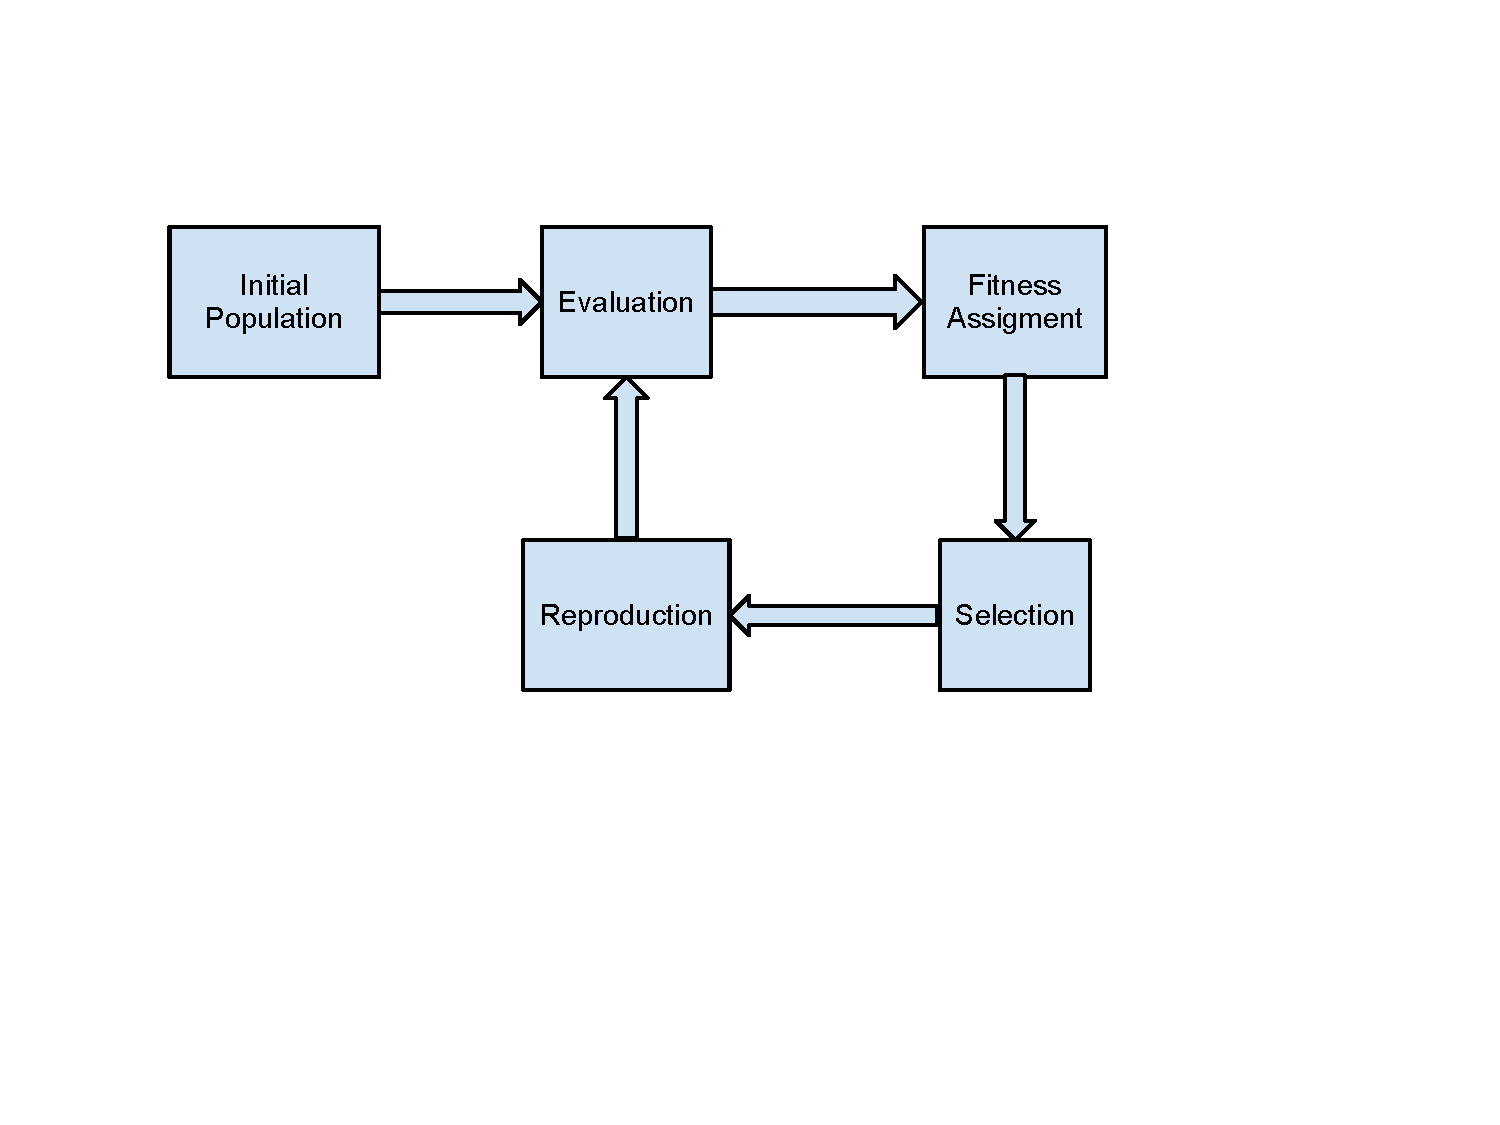
\includegraphics[scale=0.5]{img/cycle}
  \end{center}
\end{frame}

\subsection{When uses Evolutionary Algorithm?}

\begin{frame}
  \frametitle{When uses Evolutionary Algorithm?}
  \begin{block}{When...}
    \begin{itemize}
    \item We can't find a solution with classical computations,
    \item We are able to find a way to evaluate an individual.
    \end{itemize}
  \end{block}

  \begin{block}{Examples}
    \begin{itemize}
    \item Prisoner's dilemma\cite{axelrod1991},
    \item Intrusion detection in a system\cite{crosby1995},
    \item Autoparallelization\cite{walsh1996}.
    \end{itemize}
  \end{block}
\end{frame}

\subsection{Definitions}

\begin{frame}
  \frametitle{EA, GA, GP, ES... ???}
  \begin{block}{In the literature}
    \begin{itemize}
    \item When you are looking for genetic programming, you'll find a
      lot of different things.
    \item In this talk, we consider Evolutionary Algorithm as an
      umbrella term to represent techniques which use evolution.
    \end{itemize}
\end{block}

  \begin{center}
    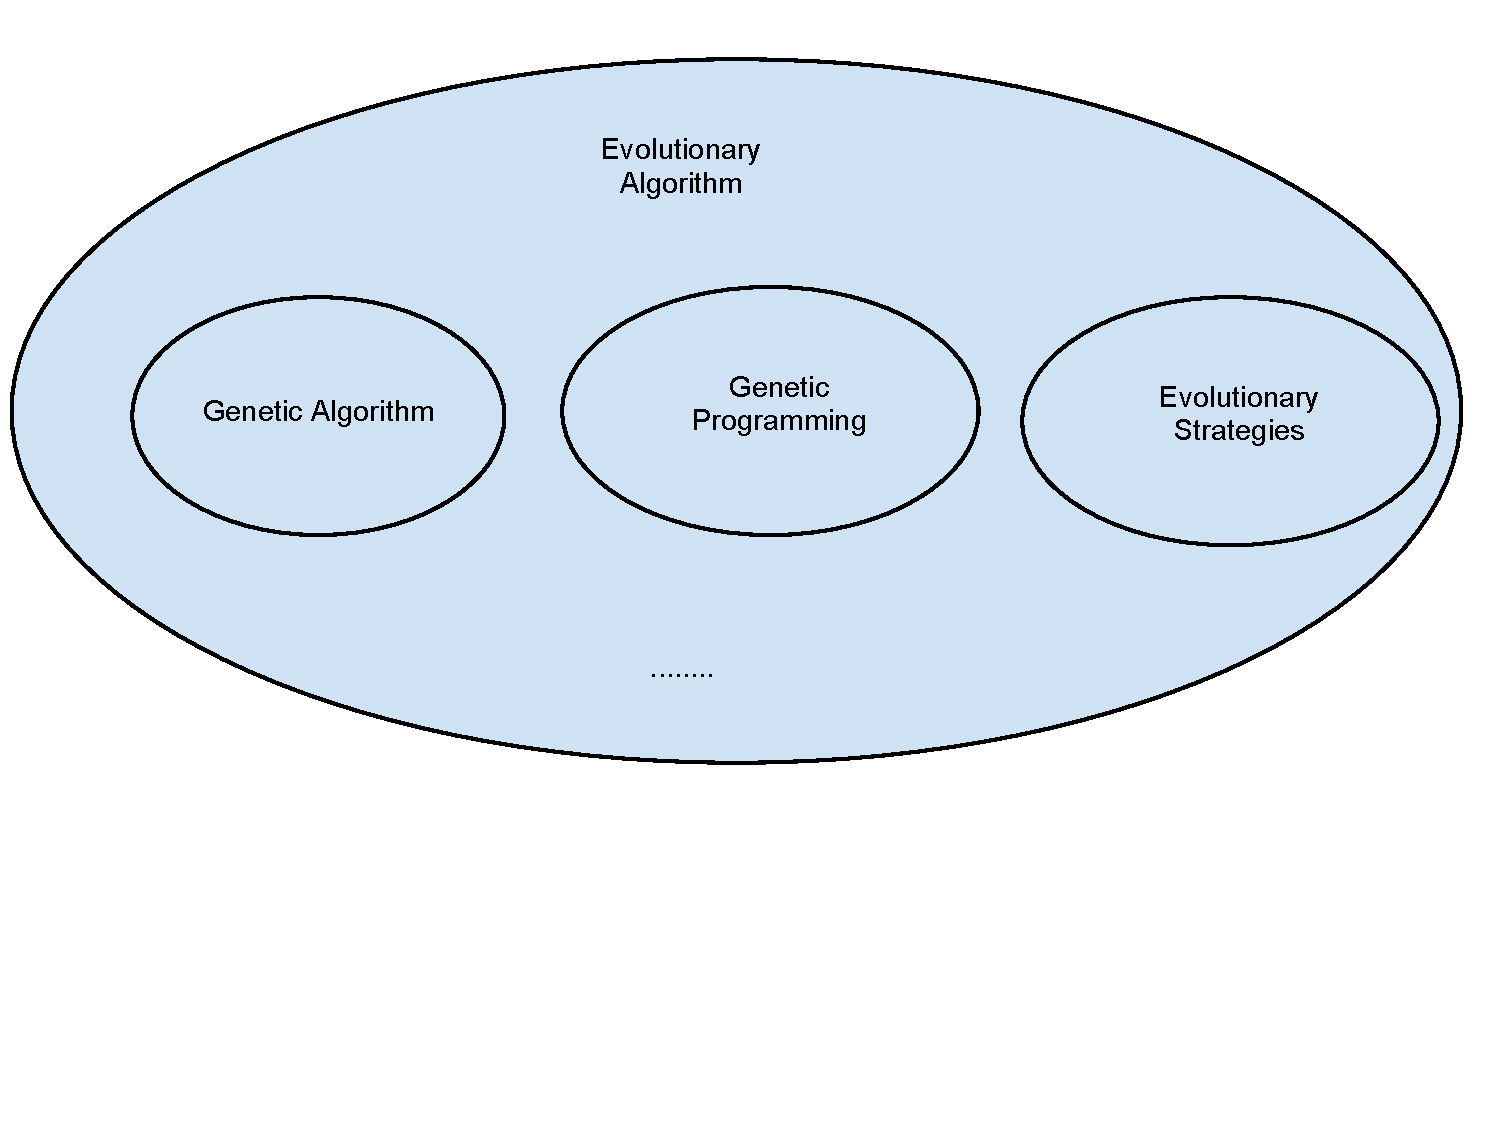
\includegraphics[scale=0.4]{img/ea}
  \end{center}
\end{frame}

\begin{frame}
  \frametitle{Genetic Algorithms}
  \begin{block}{History}
    \begin{itemize}
    \item Developed by Holland\cite{holland1992}.
    \item The original GA uses:
      \begin{itemize}
        \item fixed-length binary representation.
        \item Crossover a lot.
      \end{itemize}
    \item This model has been extended, now GA uses an alphabet (like DNA).
    \item We'll let the theoretical development for the second part.
      %% In this phrase, I mean Pierre, you have to explain the GA 1-point
      %% crossover (GP An introduction p96) and the schemata.
    \end{itemize}
  \end{block}
\end{frame}

\begin{frame}{Genetic Algorithms (cont.)}
  \begin{algorithm}[H]
    \caption{Genetic Algorithm}
    \begin{algorithmic}
      \State t := 0
      \State initPopulation P(t)
      \State evaluate P(t)
      \While {not done}
        \State ++t
        \State P' := selectParents P(t)
        \Comment{Crossover}
        \State recombine P'(t)
        \State mutate P'(t)
        \State evaluate P'(t)
        \State P := survive P', P(t)
      \EndWhile
    \end{algorithmic}
  \end{algorithm}
\end{frame}

\begin{frame}
  \frametitle{Evolutionary Strategies}
  \begin{block}{History}
    \begin{itemize}
    \item Idea started in 1960.
    \item Defined by Rechenberg\cite{Rechenberg.1975} and Schwefel\cite{Schwefel.1981}.
    \end{itemize}
  \end{block}

  \begin{block}{Characteristics}
    \begin{itemize}
    \item Only mutation.
    \item In the selection: each generation is more little than the
      precedent.
    \end{itemize}
  \end{block}
\end{frame}


\begin{frame}
  \frametitle{Evolutionary Programming}
  \begin{block}{History}
    \begin{itemize}
      \item Created in 1966, by Fogel, Owens, and Walsh\cite{fogel1966}.
    \end{itemize}
  \end{block}

  \begin{block}{Characteristics}
    \begin{itemize}
    \item Works on Finite-State Machine.
    \item Can modify: initial state, number of states, transition\dots
    \item Mutation decreases as the optimal fitness approaches.
    \end{itemize}
  \end{block}
\end{frame}


\begin{frame}
  \frametitle{Genetic Programming}
  \begin{block}{History}
    \begin{itemize}
    \item Works on program instead of parameters.
    \item Introduced by Koza\cite{Koza92}.
    \item Works on parse-tree.
    \end{itemize}
  \end{block}

  \begin{block}{Characteristics}
    \begin{itemize}
    \item Many people uses LISP.
    \item We can found assembly language too.
    \item Example: can find the function $x^2/2$.
    \end{itemize}
  \end{block}
\end{frame}

\subsection{Genetic Operators}

\begin{frame}
  \frametitle{Genetic Operators}
  \begin{block}{What is this?}
    \begin{itemize}
    \item The initial population has a very low fitness.
    \item Genetic operators make them evolves.
    \end{itemize}
  \end{block}

  \begin{block}{Who are they?}
    \begin{description}
    \item[Crossover] Mix the genome.
    \item[Mutation] Create new kind.
    \item[Reproduction] Change the population.
    \end{description}
  \end{block}

\end{frame}

\begin{frame}
  \frametitle{Crossover}
  \begin{block}{The concept}
    \begin{itemize}
    \item Mix the genome.
    \item Create new elements.
    \item There is a lot of different techniques.
    \end{itemize}
  \end{block}

  \begin{block}{Tree-based Crossover}
    \begin{itemize}
    \item Select randomly two nodes in two threes, and exchange their
      child.
    \end{itemize}
  \end{block}
\end{frame}


\begin{frame}
  \frametitle{Crossover (cont.) - Linear crossover}
  \begin{figure}[ht]
    \centering
    \visible<1-3>{
      \subfigure{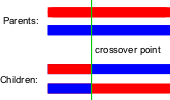
\includegraphics[width=4.5cm]{img/SinglePointCrossover}}
    }
    \visible<2-3>{
    \subfigure{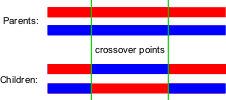
\includegraphics[width=4.5cm]{img/TwoPointCrossover}}
    }
    \visible<3>{
    \subfigure{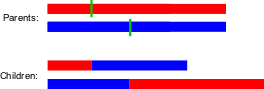
\includegraphics[width=4.5cm]{img/CutSpliceCrossover}}
  }
  \end{figure}
\end{frame}

\begin{frame}
  \frametitle{Mutation}
  \begin{block}{Concept}
    \begin{itemize}
    \item Operate on only one individual.
    \item Generally after the crossover.
    \item Low probability.
    \end{itemize}
  \end{block}

  \begin{block}{On tree structures}
    \begin{itemize}
    \item Take randomly a node, and replace its children by a new subtree
      randomly created.
    \item This subtree respects the limitation (size, depth\dots) on
      the tree.
    \end{itemize}
  \end{block}
\end{frame}

\begin{frame}
  \frametitle{Mutation (cont.)}
  \begin{block}{On linear structures}
    \begin{itemize}
    \item Take an element randomly.
    \item Apply one or more changes.
    \end{itemize}
  \end{block}

  \begin{block}{Example}
    \begin{itemize}
    \item Suppose we are in GP, ``$r_0 = r_1 + r_2$'' could become:
      \begin{itemize}
      \item $r_1 = r_1 + r_2$
      \item $r_0 = r_1 - r_2$
      \item $r_0 = r_0 + r_0$
      \item \dots
      \end{itemize}
    \end{itemize}
  \end{block}
\end{frame}

\begin{frame}
  \frametitle{Reproduction}
  \begin{block}{Concept}
    \begin{itemize}
    \item If an individual is selected, it is copied.
    \item Two versions of the same individual (unless we chose to kill
      the parents).
    \end{itemize}
  \end{block}
\end{frame}

\begin{frame}
  \frametitle{Fitness}
  \begin{block}{Concept}
    \begin{itemize}
    \item This is the function which allows to classify an individual.
    \item There is a lot of way to consider this function\dots
    \end{itemize}
  \end{block}

  \begin{block}{Examples}
    \begin{itemize}
    \item The number of matching pixels in an image matching application.
    \item The number of wall hits for a robot controlled by GP and
      learning obstacles avoidance.
    \item The number of correctly classified examples in a
      classification tasks.
    \item The money won by a GP-controlled agent in a betting game.
    \item \dots
    \end{itemize}
  \end{block}
\end{frame}

\begin{frame}
  \frametitle{The Selection Algorithm}
  \begin{block}{Concept}
    \begin{itemize}
    \item The way we select individuals.
    \item There is a lot of way.
    \end{itemize}
  \end{block}

  \begin{block}{Fitness Proposal Selection}
    \begin{itemize}
    \item Used for GA-type algorithms.
    \item Introduced by Holland\cite{holland1992}.
    \item $p_i = f_i / \sum_{j}f_j$
    \end{itemize}
  \end{block}
\end{frame}

\begin{frame}
  \frametitle{The Selection Algorithm (cont.)}
  \begin{block}{Truncation}
    \begin{itemize}
    \item Used for ES-type algorithms,
    \item Introduced by Schwefel\cite{schwefel1995},
    \item Coma-evolution: All parents died before selection,
    \item Plus-evolution: All are considered for selection,
    \item We take only the $\mu$ best individuals.
    \end{itemize}
  \end{block}

  \begin{block}{Ranking}
    \begin{itemize}
    \item Based on the fitness order.
    \item Two kind on ranking are (mainly) used, linear and exponential.
    \end{itemize}
  \end{block}
\end{frame}

\begin{frame}
  \frametitle{The Selection Algorithm (cont.)}
  \begin{block}{Tournament}
    \begin{itemize}
    \item It is a competition in a subset of the population.
    \item Participants are randomly selected.
    \item The size is a parameters of the algorithm, and allow to
      adjust the selection pressure.
    \item The winners of the tournament replaced the loser.
    \item This is a mainstream method for selection.
    \item Easy to parallelize.
    \end{itemize}
  \end{block}

  \begin{block}{Roulette wheel}
    \begin{itemize}
    \item All the population is on a contiguous segment.
    \item The size of an individual segment is proportional to its fitness.
    \item We select N times a random number (N is the number of the
      next generation).
    \item The individual whose segment spans the random number is selected.
    \end{itemize}
  \end{block}
\end{frame}


%%% Local Variables:
%%% mode: latex
%%% mode: flyspell
%%% TeX-master: "../genetic"
%%% ispell-dictionary: "en"
%%% compile-command: "cd .. && make"
%%% End:

\section{Theory}

\begin{frame}{Motivations}
  \begin{block}{Algorithmic problems}
    \begin{itemize}
      \item Stochastic
      \item Convergence
    \end{itemize}
  \end{block}

  \begin{block}{Modelisation problems}
    \begin{itemize}
      \item How to encode a problem?
      \item Size of the initial population?
      \item Mutation operator?
      \item Recombination operator?
      \item Individual selection?
    \end{itemize}
  \end{block}
\end{frame}

\subsection{Schemata Theorem}
\begin{frame}{Presentation}
  \begin{block}{Goal}
    \begin{itemize}
    \item Defined by J.Holland in 1975\cite{holland1992}.
    \item Represent a group of indidual who all share some caracteristics.
    \item One schema, two schemata ;)
    \end{itemize}
  \end{block}    

  \begin{block}{Definition}
    \begin{itemize}
    \item Defined on the alphabet: $\{0;1;\#\}$
    \item $\#$ is "Don't care": it can be 0 or 1
    \end{itemize}
  \end{block}
\end{frame}

\begin{frame}{Example and mesures}
  \begin{block}{Example}
    \begin{itemize}
    \item The schema: $H = 1\textcolor{red}{\#}10\textcolor{red}{\#}1\textcolor{red}{\#}$
    \item Represents the following individuals:
      \begin{center}
        $1\textcolor{red}{0}10\textcolor{red}{0}1\textcolor{red}{0}$,
        $1\textcolor{red}{0}10\textcolor{red}{0}1\textcolor{red}{1}$,
        $1\textcolor{red}{0}10\textcolor{red}{1}1\textcolor{red}{0}$,
        $1\textcolor{red}{0}10\textcolor{red}{1}1\textcolor{red}{1}$,
        $1\textcolor{red}{1}10\textcolor{red}{0}1\textcolor{red}{0}$,
        $\ldots$
      \end{center}
    \end{itemize}
  \end{block}

  \begin{block}{Measures}
    \begin{itemize}
      \item Order(o): number of fixed positions
      \item Defining length($\delta$): distance between the first and last defined positions.
      \item Here: $o(H) = 4$ and $\delta(H) = 5$
      \item Intuitively: schemata with low o and short $\delta$ have an higher probability of surviving from a generation to the next.
    \end{itemize}
  \end{block}
\end{frame}

\begin{frame}{Graphical representation}
  \begin{center}
    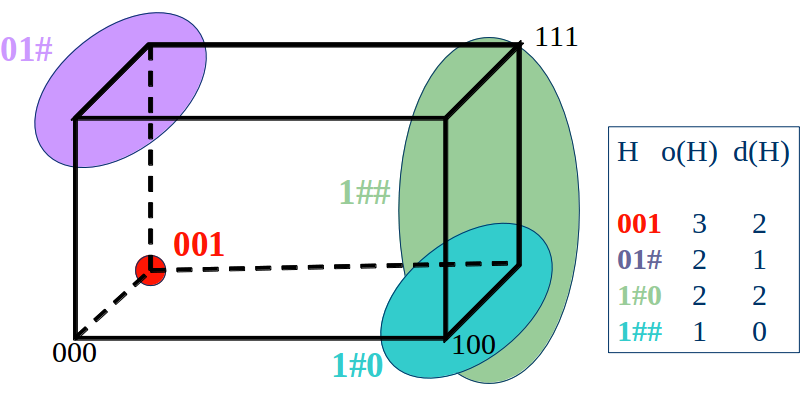
\includegraphics[scale=.4]{img/schema}
  \end{center}
\end{frame}

\begin{frame}{Possible evolutions : selection}
  \begin{block}{Hypothesis}
    \begin{itemize}
    \item Assume a fitness proportional reproduction
    \item $$\mathds{P}(x,t+1) = \frac{f(x)}{\bar{f(t)}}$$
    \end{itemize}
  \end{block}

  \begin{block}{Transmission of a schema}
    $$\begin{array}{lll}
      \mathds{P}(H,t+1) & = & \sum\limits_{x \in H} \frac{f(x)}{\bar{f(t)}}\\
      & = & m(H,t) \times \frac{f(H,t)}{\bar{f(t)}}\\
    \end{array}$$
  \end{block}
\end{frame}

\begin{frame}{Disruptions}
  \begin{block}{Mutation}
    \begin{itemize}
    \item bit-wise mutations with probability $p_m$
    \item Mutation events are independant
    \item $\mathds{P}_{Smuta}(H) \geq (1 - p_m)^{o(H)}$
    \end{itemize}
  \end{block}

  \begin{block}{Crossover}
    \begin{itemize}
      \item One point crossover with probability $p_c$
      \item l - 1 possible crossover points
      \item $\mathds{P}_{Scross}(H) \geq (1 - p_c \times \frac{\delta(H)}{l - 1})$
    \end{itemize}
  \end{block}
\end{frame}

\begin{frame}{Schema theorem}
  \begin{block}{Theorem}
    $$E(m(H,t+1)) \geq \underbrace{m(H,t) \times \frac{f(H,t)}{\bar{f(t)}}}_{\mathds{P}(x,t+1)}
    \underbrace{\times (1 - p_c \times \frac{\delta(H)}{l-1})\vphantom{\frac{f(H,t)}{\bar{f(t)}}}}_{\mathds{P}_{Smuta}}
    \underbrace{\times (1 - p_m)^{o(H)}\vphantom{\frac{f(H,t)}{\bar{f(t)}}}}_{\mathds{P}_{Scross}}$$
  \end{block}
\end{frame}

\begin{frame}{Extension to GP}
\end{frame}

\begin{frame}{Building Block hypothesis}
\end{frame}

\begin{frame}{Price's theorem}
\end{frame}

\begin{frame}{Limitations}
\end{frame}

\begin{frame}{Conclusion}
\end{frame}

\section{Application}

\subsection{Prerequisites}

\begin{frame}{MMORPG}
  \begin{block}{Definition}
    \begin{itemize}
    \item Massively Multiplayer Online RolePlaying Game
    \item Persistent World
    \end{itemize}
  \end{block}

  \begin{block}{Environment properties}
    \begin{itemize}
    \item Monsters
      \begin{itemize}
      \item Agressive
      \item Passive
      \end{itemize}
    \item

    \end{itemize}
  \end{block}

  \begin{block}{Purpose}
    \begin{itemize}
    \item Kill monsters
    \item Survive
    \end{itemize}
  \end{block}
\end{frame}

\begin{frame}{Openkore}

  \begin{block}{Definition}
    \begin{itemize}
    \item Program (Bot) which simulate a player in a MMORPG (here Ragnarok Online)
    \item Take a configuration file (so the bot is scriptable) as input
    \end{itemize}
  \end{block}

  \begin{block}{Why this application ?}
    \begin{itemize}
    \item There is a complex environment where the bot has life points, experience, position and a lot of other properties
    \item The bot is subjected to virtual physical constraints therefore we can have a lot of different fitness functions
    \item A lot of parameters available to customize the bot behaviour
    \item Easy to implement
    \end{itemize}
  \end{block}

\end{frame}
\subsection{Principle}

\begin{frame}{Parameters}

  \begin{block}{Parameters / Genes}
    \begin{itemize}
    \item The reaction of the bot when he sees an enemy:
      \begin{itemize}
      \item Attack
      \item Run away
      \item etc
      \end{itemize}
    \item A total of N * 6 parameters where N is the number of monsters on the map
    \end{itemize}
  \end{block}

  \begin{block}{Example}
    TODO: Display parameters for one bot
  \end{block}

\end{frame}

\begin{frame}{Repopulation}
  \begin{block}{Selected fitness functions}
    \begin{itemize}
    \item Life points : Try to minimize the life points lost in a round
    \item Experience points : Try to maximize the experience points acquired in a round
    \item Hybrid : Try to maximize the function $f = \frac{exp}{life} $
    \end{itemize}
  \end{block}

  \begin{block}{Selected reproduction}
    \begin{itemize}
    \item Mutation
    \item Crossover
    \end{itemize}
  \end{block}
\end{frame}

\subsection{Demonstration}

\begin{frame}{Demonstration}
  Demonstration !
\end{frame}

\subsection{Result}

\begin{frame}{Result}
  TODO: Insert results for different fitness functions here
\end{frame}


\begin{frame}
  \frametitle{Conclusion}
  \begin{block}{Evolutionary algorithm}
     \begin{itemize}
     \item Powerful tool
     \item Used in complex problems
     \item Hard to modelize problems
     \end{itemize}
  \end{block}

  \begin{block}{Theory}
    \begin{itemize}
    \item Theoretical basis for GA and GP
    \item Hard to understand
    \item A lot of controversies
    \end{itemize}
  \end{block}
\end{frame}

\begin{frame}
  \frametitle{Questions?}
  \begin{center}
    
\includegraphics[scale=0.7]{img/questions.jpg}
  \end{center}
\end{frame}

\section{References}

\begin{frame}[allowframebreaks]{Bibliography}
  \footnotesize
  \bibliographystyle{unsrt}
  \bibliography{biblio}
\end{frame}

\end{document}
